\documentclass[conference]{IEEEtran}
\IEEEoverridecommandlockouts

% The preceding line is only needed to identify funding in the first footnote. If that is unneeded, please comment it out.
\usepackage{cite}
\usepackage{amsmath,amssymb,amsfonts}
\usepackage{algorithmic}
\usepackage{graphicx}
\usepackage{textcomp}
\usepackage{xcolor}
\usepackage{multirow}
\usepackage{hyperref}
\usepackage{breakurl}
\usepackage{float}
\usepackage{booktabs}
\def\BibTeX{{\rm B\kern-.05em{\sc i\kern-.025em b}\kern-.08em
    T\kern-.1667em\lower.7ex\hbox{E}\kern-.125emX}}
% special commands
\usepackage{enumitem}
\setlist{topsep=1em, itemsep=1em}

\begin{document}

% paper starts
\title{ECS 171: Deep Learning for Diabetes Risk\\
}

\makeatletter
\newcommand{\linebreakand}{%
  \end{@IEEEauthorhalign}
  \hfill\mbox{}\par
  \mbox{}\hfill\begin{@IEEEauthorhalign}
}
\makeatother

\author{
    \IEEEauthorblockN{\textbf{Arjun Ashok*}\thanks{* Corresponding author.}}
    \IEEEauthorblockA{\textit{College of Engineering, Letters \& Science} \\
    \textit{University of California, Davis}\\
    Davis, United States of America \\
    arjun3.ashok@gmail.com}
%
\and
%
    \IEEEauthorblockN{Taha Abdullah}
    \IEEEauthorblockA{\textit{College of Engineering} \\
    \textit{University of California, Davis}\\
    Davis, United States of America \\
    tmabdullah2002@gmail.com}
%
\linebreakand
%
    \IEEEauthorblockN{Tej Sidhu}
    \IEEEauthorblockA{\textit{College of Engineering} \\
    \textit{University of California, Davis}\\
    Davis, United States of America \\
    tsidhu@outlook.com \\
    ORCID: 0000-0002-3496-2211}
    
\and
    \IEEEauthorblockN{Devon Streelman}
    \IEEEauthorblockA{
        \textit{College of Letters and Science} \\
        \textit{University of California, Davis}\\
        Davis, United States of America \\
        devonstreelman@gmail.com
    }
%
\and
%
    \IEEEauthorblockN{Ayush Tripathi}
    \IEEEauthorblockA{\textit{College of Engineering} \\
    \textit{
        University of California, Davis}\\
        Davis, United States of America \\
        atripathi7783@gmail.com
    }
}

\maketitle
\thispagestyle{plain}
\pagestyle{plain}

\begin{abstract}
Diabetes is one of the most prevalent chronic diseases to date in the world, with numerous harmful long-term effects on the body. As a result, diagnosis of this disease is crucial to prevent damaged organs and blood vessels, which often lead to kidney failure, heart attack, and stroke. Due to a lack of healthcare access across the world, over 30\% of people with diabetes are undiagnosed.  Thus, easy-to-access and accurate identification of this disease utilizing information readily available to undiagnosed individuals is essential to ensure that they get the necessary care. Throughout this research paper, we employ a deep learner to efficiently and effectively diagnose diabetes. The most common type of diabetes, Type 2 Diabetes, is completely preventable. Hence, we also use a linear approximator to identify diabetes risk factors based on an individual’s lifestyle. The classifier we created has a diabetes-free F1 score of 0.821 and a diabetes F1 score of 0.425. We claim this outperforms all the F1 scores of prior work with our dataset. \\
\end{abstract}

\begin{IEEEkeywords}
Deep Learning, Classification, Tabular, Diabetes, Risk Analysis
\end{IEEEkeywords}

\section{Introduction and Motivation}\label{sec:intro}
    \subsection{Background on Diabetes \& Research Questions}
Diabetes is a chronic disease that occurs when insulin does not properly regulate the body’s blood sugar. This occurs if the pancreas fails to produce enough insulin, or if the body cannot effectively use the insulin it is currently producing. The most common course of treatment for diabetic individuals is insulin injections, which can be supplemented with or replaced in certain situations with other medications that can lower blood sugar\cite{b2}. \\
\indent Diabetes can impede an individual’s ability to complete normal activities and the number of people with diabetes is increasing each year. As of 2021, there are over 537 million individuals with diabetes in the world and the number is projected to hit 643 million in 2030\cite{b4}. Furthermore, around 2 million people die from diabetes or diabetes-related complications each year\cite{b2}, with 6.1 million people dying from diabetes or diabetes-related complications in 2021\cite{b4}. \\
\indent The current statistics paint a very bleak picture for the outlook of diabetes. Luckily, the most common type of diabetes, Type 2 Diabetes, is completely preventable. If an individual can identify risky behaviors early on, they can adjust their lifestyle to prevent the onset of diabetes. These findings motivated our first question:

\begin{enumerate}[label=\roman*.]
    \item given an individual’s lifestyle, can we identify specific risk factors for diabetes? \label{itm:rq1}
\end{enumerate}

\indent Furthermore, when doing our background research on diabetes, we learned that diabetes is often undiagnosed. For instance, 54\% of adults living with diabetes in Africa are undiagnosed, 36\% in Europe, and 30\% in the Middle East, with comparable numbers in other regions of the world\cite{b4}. A large reason for this underdiagnosis is that there is a lack of access to adequate medical facilities, preventing individuals from taking the blood test necessary for a diagnosis\cite{b2}. This development prompted us to add another question to our risk factor assessment.

\begin{enumerate}[label=\roman*.]
    \setcounter{enumi}{1}
    \item given an individual’s lifestyle, can we accurately assess whether they are diabetes-free, pre-diabetic, or diabetic? \label{itm:rq2}
\end{enumerate}


\subsection{Paper Outline}
To answer these questions, we decided to implement a machine-learning model that can classify individuals as diabetes-free, pre-diabetic, or diabetic, addressing RQ \ref{itm:rq2}. We then use a generalized linear model approximation of the neural network to identify the individual’s diabetes risk factors, addressing RQ \ref{itm:rq1}. The paper starts by analyzing existing literature and projects to provide a better idea of what state-of-the-art models and techniques researchers currently use to solve similar problems or in similar domains. After this analysis, we can begin to develop our model. We start by finding a dataset and performing exploratory data analysis to understand the data’s characteristics. In this step, we also pre-processed our data to ensure its suitability for model training. After we describe all the preparatory steps, we focus on the methodology we used to select important features, engineer them, and build out our shortlist of models. The models we build and test include gradient boosting, deep neural networks, and logistic regression. We then evaluate these models in the context of our questions and see if we have developed an effective solution.

\section{Literature Review}\label{sec:litreview}
To understand the state of the art in diabetes prediction (without the use of blood sugar/glucose), we evaluated three key areas:

    \begin{enumerate}
        \item State-of-the-Art [SOTA] for diabetes modeling and prediction to ensure we're using the correct strategies for our specific context
        \item State-of-the-Art [SOTA] for classification in healthcare to serve as a comparison and allow us to make a more generalized pipeline
        \item State-of-the-Art [SOTA] in tabular classification models, specifically XGBoost vs Deep Neural Networks, so we employ the best modeling techniques
    \end{enumerate}

\subsection{Diabetes Modeling \& Predictions }

\subsubsection{Introduction}
The paper\cite{b5} discusses various machine learning models that have been explored to enhance the prediction accuracy of diabetes, through utilizing diverse datasets and sophisticated feature selection techniques.

\subsubsection{Data Sources and Preprocessing}
The primary dataset used in diabetes prediction studies is the open-source Pima Indian dataset. The Pima Indian dataset is widely used due to its availability and comprehensive nature, including features such as pregnancies, glucose, blood pressure, skin thickness, insulin, BMI, age, and diabetes pedigree function. 

\subsubsection{Machine Learning Models}
Several machine learning models were employed to predict diabetes, each with varying degrees of accuracy and performance. The Random Forest model demonstrated an accuracy of 90\% in some studies, consistently showing high performance due to its ability to handle diverse datasets and reduce overfitting. Decision Tree models, on the other hand, exhibited an accuracy ranging from 73\% to 79\%, depending on the dataset and preprocessing techniques used. While Decision Trees generally have lower accuracy compared to ensemble methods, they are still valuable for preliminary analysis.
Logistic Regression models achieved an accuracy between 75\% and 77\% with hyperparameter tuning, offering moderate accuracy and serving as a useful baseline model. Finally, the XGBoost model attained an accuracy of 81\% when combined with the ADASYN technique. 


\subsubsection{Results and Discussion}
The XGBoost classifier, particularly when combined with the ADASYN approach, achieved the second highest performance with an 81\% accuracy rate. This highlights its strength in managing class imbalance and complex data patterns. In contrast, the Random Forest model exhibited the highest accuracy of 90\% in some studies, though this was dataset-dependent.

The variability in performance across models emphasizes the need for careful selection based on dataset characteristics and specific problem requirements. For instance, while Logistic Regression and Decision Tree models provide interpretability and ease of use, they may fall short in accuracy compared to ensemble methods like Random Forest and XGBoost.

\subsubsection{Conclusion}
The study underscores the significant efficacy of various machine learning models in predicting diabetes, with XGBoost emerging as the most precise and consistent model. It is important to note that the accuracy percentages may differ when applied to datasets from the United States, as the patient demographics and feature impacts can vary geographically. For instance, age, BMI, and blood glucose concentration were key predictive features in this study, but their influence might differ in U.S. datasets due to varying population characteristics and health factors.



\subsection{Classification in Healthcare}
In the literature\cite{b2}, we found that the diagnosis of heart disease through machine learning has taken similar approaches to ours. Li et al. created their models using the Cleveland Heart Disease dataset. Throughout their preprocessing, the researchers removed attribute missing values and scaled their data with both a standard scalar technique and the min-max scalar technique.

\subsubsection{Model Output}
The researchers applied various classification models to the data, including linear regression (LR), Kth nearest neighbor (KNN), artificial neural network (ANN), support vector machine (SVM), naive Bayes (NB), and decision trees (DT). Additionally, they used a variety of feature selection algorithms, including Relief, MRMR (Maximum Relevance - Minimum Redundancy), LASSO, and LLBFS (Layer-Wise Learning Based Feature Selection). After extensive testing of each classification model with the respective feature selection algorithm, the proposed algorithm was FCMIM (Fast Conditional Mutual Information Maximization) because of its performance compared to the other feature selection algorithms. The researchers reported the accuracy of the models using FCMIM, with LR at 88.67\%, KNN at 82.11\%, ANN at 75.23\%, SVM at 92.37\%, NB at 86.01\%, and DT at 79.12\%. The model and feature selection with the best results was FCMIM-SVM with 92\% accuracy.

\subsubsection{Conclusions}
This study is significant to our research as it demonstrates the effectiveness of various machine learning models and feature selection algorithms in diagnosing heart disease. The high accuracy achieved by the FCMIM-SVM model highlights the potential for advanced feature selection techniques to enhance the performance of machine learning models in medical diagnoses. Diagnosing a general medical condition like heart disease has broader implications for diagnosing other diseases, such as diabetes. The methodologies and insights gained from heart disease diagnosis can be applied to diabetes diagnosis, potentially improving accuracy and early detection. Both conditions share common risk factors and comorbidities, making the transfer of diagnostic techniques between them highly relevant. By leveraging similar machine learning models and feature selection algorithms, we can enhance our ability to identify and manage diabetes, ultimately leading to better patient outcomes.


\subsection{Tabular Classification }
\subsubsection{Introduction}

The paper\cite{b7} compares 11 different studies that utilize DNN for tabular datasets. Then the DNN model is trained on other tabular datasets and the results are noted. An XGBoost model is created and trained on all the same datasets as DNN. The paper then compares DNN and XGBoost on the original dataset and on the other datasets.


\begin{table}[ht]
\caption{Relative Performance in Comparison to Best Model on Other Datasets (Lower Value is Better)}
\begin{center}
\begin{tabular}{|c|c|}
\hline
\textbf{Model} & \textbf{Average Relative Performance (\%)} \\
\hline
XGBoost & 3.34 \\
NODE & 14.21 \\
DNF-Net & 11.96 \\
TabNet & 10.51 \\
1D-CNN & 7.56 \\
\hline
\end{tabular}
\end{center}
\end{table}

\subsubsection{Analysis}
The analysis reveals that deep models are less accurate and precise on newly introduced datasets compared to the XGBoost model. The performance of deep models is highly sensitive to the specific dataset, making them useful for creating classifiers tailored to particular datasets, such as our diabetes dataset. However, they underperform when generalized to other datasets, which is why we included the XGBoost model in our package for broader applicability in disease and condition classification. The differences in performance are largely due to hyperparameter optimization. Without proper optimization, XGBoost generally outperforms deep neural networks (DNNs), but with well-tuned hyperparameters for a specific dataset, DNNs can surpass XGBoost.









\section{Dataset \& Exploratory Data Analysis}\label{sec:eda}
The dataset we utilized for our project is the Diabetes Health Indicators dataset generated by Alex Teboul in 2021, a cleaned version of the BBRFSS 2015 dataset already created by the Center of Disease Control and Prevention. We chose this dataset because it presented a challenge with multi-class target labels and a severe imbalance. Its limited correlation across features and cleanliness meant it had potential for downstream interpretation of data and for fair model applicability. There was also a plethora of data, with 253, 680 observations of 22 features.\\\\
    
    \begin{figure}[h]
        \centering
        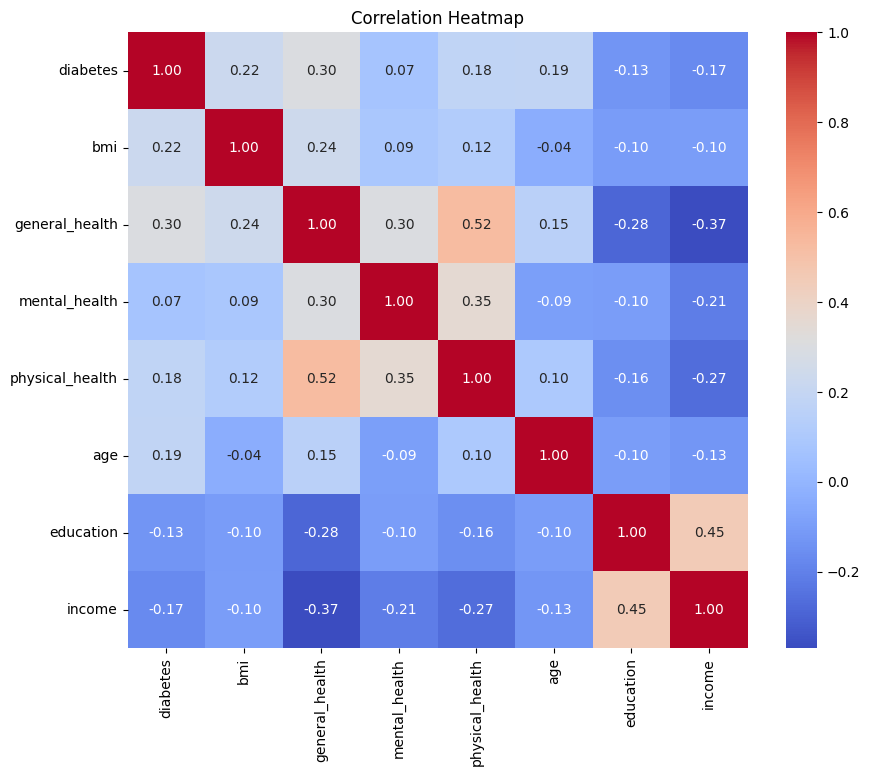
\includegraphics[scale=0.39]{correlations2.png}
        \caption{Correlation Heatmap for our Features}
        \label{fig:outliersBMI}
    \end{figure}


    \begin{figure}[h]
        \centering
        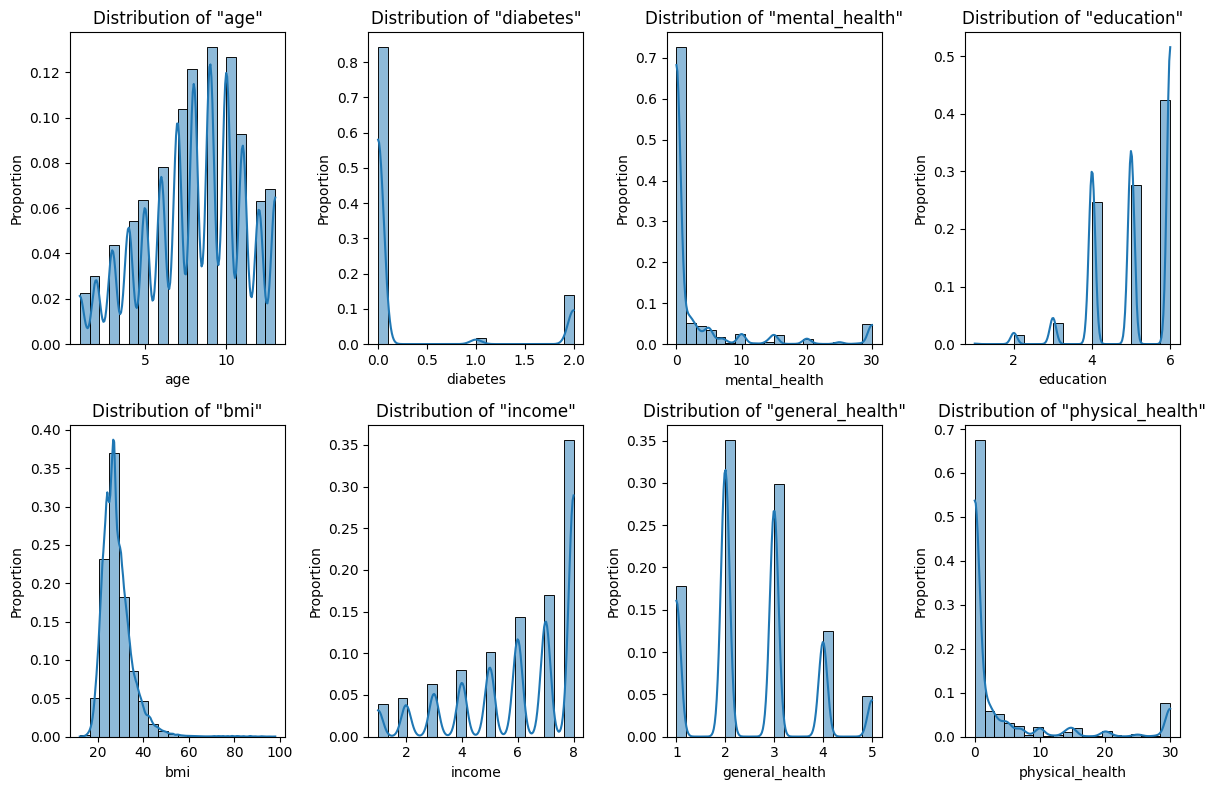
\includegraphics[scale=0.3]
        {dataplots.png}
        \caption{Data Distributions}

        \label{fig:bmi standardized}
    \end{figure}

    
Throughout EDA we were sure to note the following:

\subsection{Data Cleaning}
During our initial evaluations during out EDA, we noticed the data was quite clean and there was a minimal amount of work necessary to get the data to the acceptable level. What was needed, however, was operations such as outlier detection, skew visualization, data transformation (one hot encoding) and standardization to get our data to an acceptable level for our classification algorithms. 

\subsection{Outliers}
Detection of outliers was streamlined through a outlier detection algorithm using the IQR method, with outliers being values beyond 1.5 * IQR. Outliers were then visualized by plots of distribution of the features, highlighting outliers in red and eliminating them if necessary.

    \begin{figure}[h]
        \centering
        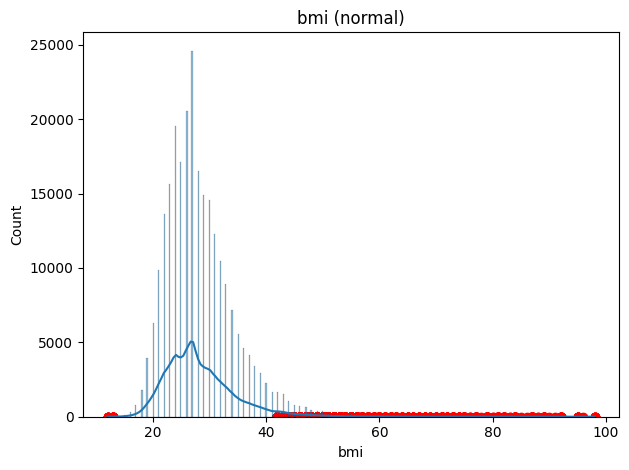
\includegraphics[scale=0.39]{outliersBMI.png}
        \caption{Outliers are highlighted in red.}
        \label{fig:outliersBMI}
    \end{figure}
% \subsection{Data Skew}
% Upon visualization of the data, we found that there is a large imbalance of target variables, such as an overabundance in non-diabetes at 84\% and diabetes only sitting at 2\%. We resolve this imbalance via two approaches, one in the data pre-processing stage and one in the modeling stage (Section \ref{sec:methodology}, Section \ref{sec:eval}).

\subsection{Feature Analysis}
Throughout our EDA, we noticed numerous categorical features with text representation. In order for these features to be included for model evaluation, we found it necessary to implement One-Hot encoding. If the feature is discovered to be ordinal we may assume a linear relationship and avoid encoding in any form because if its relationship with each level. Despite this, if there is an ordinal feature that a linear relationship cannot be assumed, we can choose to one-hot encode. With nominal features, we one-hot encode to preserve categorical nature, satisfy algorithmic requirements, and handle nominal data. 

\subsection{Distribution Imbalance}
During our analysis we noticed how there is significantly more non-diabetes observations that diabetes observations. In order to stray from imbalanced training and bias down the line, we chose to Up-sample the diabetes observations.

    \begin{figure}[h]
        \centering
        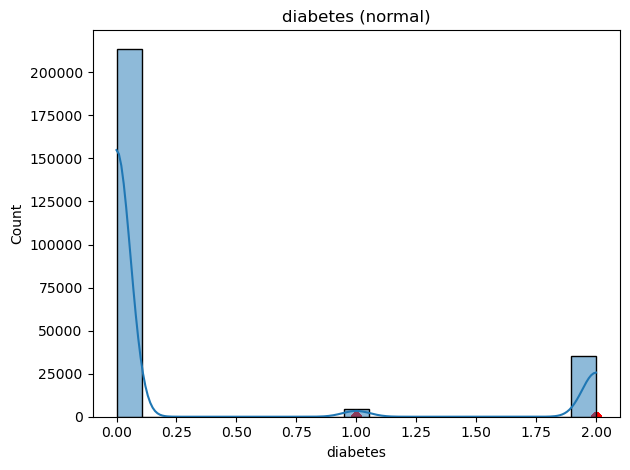
\includegraphics[scale=0.39]{diabetes.png}
        \caption{Distribution of Classes}
        \label{fig:diabetes distribution}
    \end{figure}

\subsection{Standardization}
Due to the variety in data creating difficult comparisons, we chose to standardize the data. We decided to standardize with Z-score. Standardization was necessary to ensure performance was not affected by imbalanced data, possibly resulting in biased predictions towards the majority class.

    \begin{figure}[h]
        \centering
        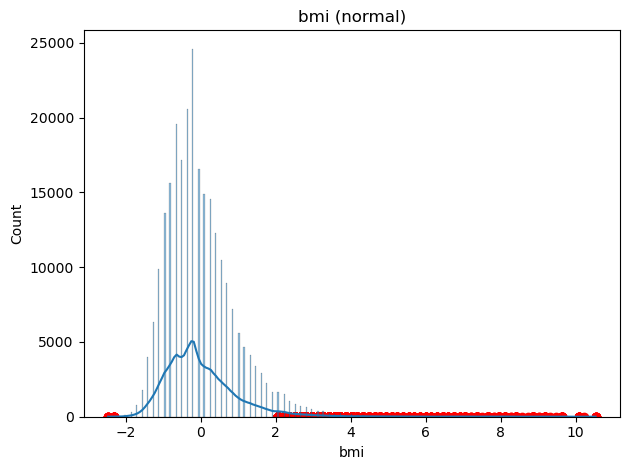
\includegraphics[scale=0.39]
        {bmi_standardized}
        \caption{With Z score standardization, bias in classification will be minimized.}

        \label{fig:bmi standardized}
    \end{figure}





\section{Methodology}\label{sec:methodology}
    \subsection{Feature Engineering}
    Although the dataset was initially quite clean, the features themselves contained some nuances that warranted further consideration:

    \begin{enumerate}[label=\roman*.]
        \item \textit{Encoding}: although already encoded, the dataset's inclusion of several ordinal features motivated consideration of one-hot encoding for non-dichotomous (binary) variables. We eventually concluded that although the relationship between each level in the ordinal variables may not be linear, the model we use downstream will be able to approximate this non-linear relationship; thus we can avoid increasing dimensionality with little opportunity for payoff.
    
        \item \textit{Normalization}: generally speaking, normalization can  boost performance of several classes of models. However, given the feature-set is primarily made up of ordinal and nominal variables, standardization could potentially mislead the model. With some experimentation, we determined that the different scales for ordinal variables and presence of some numeric variables motivates the use of scaling for those respective features. We are careful to note here that any scaling applied during training was applied during testing and downstream prediction to ensure the model saw the same type of data, especially for non-decision tree based models.

        With regards to min-max versus z-score standardization, our literature review revealed that z-score normalization tends to outperform min-max scaling in this domain. Thus, to reduce the amount of computation (i.e. combinations of parameters to test), we chose to \textit{exclusively} z-score normalize.
        
        \item \textit{Class Imbalance}: with $\sim$84\% of labels in the Diabetes-Free class, $\sim$15\% of labels in the Diabetes class, and $\sim$1\% of labels in the Pre-Diabetes class, the class imbalance stuck out as one of the key issues in the dataset. To counteract this, we experimented with a few methods in the pre-processing and modeling phases (further discussed in Section \ref{sec:imbalance}).

        To remedy the imbalance through data pre-processing, we experimented with two up-sampling strategies: (1) \textit{SMOTE} (Synthetic Minority Oversampling Technique) and (2) \textit{bootstrapping}. We ultimately decided against downsampling as an alternative since the Pre-Diabetes class would be a significant limiting factor; the only valid approach with downsampling would be to convert the problem into a binary classification of Diabetes-Free or not. Given our aim of a more detailed risk breakdown downstream, we opted to keep the Pre-Diabetes label and upsample instead.
        
        SMOTE leverages a nearest-neighbors approach to interpolate between minority samples, thus generating unique enough data to train on while preserving a high likelihood of belonging to the minority class. Since the majority of the features were ordinal or nominal, we had to employ some heuristic rounding techniques to ensure the synthetic data followed the normalization scheme we introduced.
        
        Bootstrapping, on the other hand, artificially duplicates minority label observations via the bootstrap process (i.e. sampling with replacement).
        
        Bootstrap, naively, aims to avoid a severe bias towards the majority label simply by penalizing the model for biasing against minority label (via increased loss), but it lacks the underlying information about the minority class that SMOTE provides. Coupled with case-studies (Figure \ref{fig:stratcomparison}) on the downstream performance with either strategy, we ultimately utilized SMOTE as our sole upsampling strategy.
    \end{enumerate}

    \subsection{Feature Selection}
    Given our dataset contained 22 features, many of which described similar patient characteristics, it was essential to conduct feature selection. Our approach to feature selection was four-fold:
    
    \begin{enumerate}[label=\roman*.]
        \item \textit{Collinearity}: the more related features are (in a linear manner), the more likely they are to be redundant. The lower the collinearity, the more unique the information they provide is; i.e., lower is better.
        
        \item \textit{Target Correlation}: the higher the trend between the target feature and every feature, the more likely they will be able to contribute the model’s eventual predictive power. As such, higher is better.
        
        \item \textit{Regularized Regression}: if we utilize some sort of penalty during regression modeling on the feature weights (especially with LASSO), we can conduct feature selection by removing any features whose weights are very close to zero; if any features aren’t weighted by near-zero coefficient, we can still
        use the information about their weights to determine which features provide relatively higher or lower utility. 
        
        Notice, this feature-selection must be done with scaled/standardized data since lower scales will be penalized arbitrarily more by design of LASSO/Ridge. Notice, lower scaled features require a larger coefficient to compensate for its scale relative to higher scale features. As such, all features must be on approximately the same scale to avoid unnecessarily selecting out features. In this metric, the lower the coefficient, the worse its utility is. We also employed Elastic-Net, i.e. a linear combination of the LASSO and Ridge penalty, to  more effectively draw out important features.
        
        We did also consider employing XGBoost/Random Forests to conduct feature selection primarily due to its popularity in SOTA papers \cite{b7}. Ultimately, the limited non-linearity/complexity that these models have, lack of direct interpretability, and increased computation swayed us towards using regularized regression instead.
        
        \item \textit{Context-Driven Selection}: the final step is to consider the actual context of what we are predicting to determine what features are redundant, irrelevant, or otherwise not that  useful during the modeling process. We combine this analysis with the others to cross-check that even if no \textit{linear} relationship is present, we are not removing features unnecessarily (especially in processes i. and ii.). 
        
    \end{enumerate}
    
    With this multi-faceted approach, we determined two features that seemed to under-perform in all of these tests relative to the other features. Combined with our manual pruning and considering the context of the prediction, we decided that Difficulty Walking (dichotomous) and Smoker (dichotomous) are both redundant and don’t contribute enough to justify their inclusion. However, we do collect this data in our user interface to allow future adjustments to the model and features without having to change the front end.
    
    There were other features that were not perfect throughout all tests, but given that we had a large dataset and no surefire way to determine non-linear relationships (even Principal Component Analysis fails with very non-linear trends \cite{b5}), we opted to err on the side of keeping the features rather than discard unnecessarily.
    
    \subsection{Modeling}
        \subsubsection{Model Architectures}
        Based on our literature review and exploratory data analysis, we concluded that (1) \textit{Gradient Boosting} (XGBoost), (2) \textit{Deep Neural Networks} (DNN), and (3) Logistic Regression (w/ Ridge, LASSO, or Elastic-Net) would likely perform the best. These models not only are able to model complex, non-linear relationships fairly well, but are also deemed the state of the art in this domain \cite{b2}.

        \subsubsection{Overfitting Remediation}
        Overfitting was a major concern for the Deep Neural Network in particular since ensemble techniques like Gradient Boosting are unlikely to overfit (even with a large number of sub-predictors) and Logistic Classifiers proved to be quite effective with regularization penalties \cite{b7}.
        
        In particular, we limited the depth of the sub-predictors and the number of features considered per node split for the Gradient Boosting Classifier. For the Logistic Classifier, a combination of L1 and L2 regularization, i.e. Elastic-Net, proved to be very effective and even allowed for feature-selection post data pre-processing. The validation accuracy of both were quite stable with these parameters set.

        Accordingly, we employed a few special strategies to encourage the Deep Neural Network to generalize as well:

        \begin{enumerate}[label=\roman*.]
            \item \textit{Early-Stopping}: to avoid overfitting the train set, we constantly measure a validation loss and choose the most generalizable model during training. This involves tracking the best model's performance while keeping a patience tracker (i.e. a counter that allows for some leeway in the number of epochs without improvement in the case of momentum carrying the model over a saddle-point or local minimum).

            \item \textit{Dynamic/Scheduled Learning Rate}: to converge faster and avoid saddle points, a learning rate scheduler can be utilized to slowly taper off the step size and momentum during training. Scheduler variants include functions of validation loss, epoch number, etc. Although this technique is promising, the high rate of reproduction in our results meant that our model was consistently converging onto a set of optimal weights. In other words, we conducted multiple trials of the same architecture with a different (random) initialization of weights, and the end performance was consistent. The implication here being that learning rate/momentum scheduling \textit{likely} wouldn't affect the convergence since the configuration seemed to optimize effectively each time.

            Part of this convergence efficacy was also from the choice of optimizer, ADAM (ADAptive Moment Esetimation), a form of momentum-based gradient descent that efficiently approximates gradients and avoids local minima.

            \item \textit{Dropout Layers}: rather than L1 or L2 regularization, we opted for dropout layers to enable larger architectures (i.e. more hidden layers and nodes per layer) and therefore more complexity without sacrificing as much on generalizability (since dropout isn't applied during prediction).
        \end{enumerate}

        \subsubsection{Class Imbalance [Biased Predictor]}\label{sec:imbalance}
        To address the aforementioned target label imbalance, we had the option of targeting the model itself. Specifically, by modifying the loss function that weighed the minority labels proportionally more than the majority label, we could achieve a similar effect to the up-sampling techniques. However, since no new information is gained by the model regarding these classes, the end result is a set of weights very similar to the bootstrapping approach--i.e., a predictor that isn't biased in its output, but hasn't learned enough to correctly predict the minority output labels. This can be visualized in Figure \ref{fig:stratcomparison}. As such, we concluded that SMOTE would be the optimal remedy to the class imbalance.

        \subsubsection{Thresholding}
        With regards to label prediction and thresholding, we felt it best to minimize the number of false negatives. In our context, a false positive would only motivate medical check-ups which only serves to help the user seek necessary medical intervention. A false negative, however, provides a sense of security that incentivizes not seeking treatment and potentially neglecting to address any underlying issues. We would rather push unnecessary check-ups than risk letting a disease grow worse.

        \subsubsection{Hyper-Parameter Optimization}
        Hyper-parameter optimization is notorious for its computational expense to conduct, and our context was no exception. Deep Neural Networks and Gradient Boosting are computationally expensive to train a single instance of (80 minutes on average), let alone test many different configurations. With these computational limits in mind, we tried two main techniques for the optimization:

        \begin{enumerate}[label=\roman*.]
            \item \textit{Grid-Search}: after some initial trials to understand the model performance, we set the limits of a parameter space worth further investigating and drew patterns between each hyper-parameter and the downstream performance. This was primarily helpful for the Gradient Boosting and Deep Neural Network classifiers, but not so much the logistic classifier since its performance was quite stable.
            
            \item \textit{Heuristic Search}: a manual approach where we observe the change a given feature makes and adjust other parameters accordingly. We utilized the grid-search to inform us of hyper-parameter-wise performance gains to eventual arrive at a set of combinations that performed best.
            
            Notice that less computation is required than in grid-search since we heuristically rule out a lot of options. For example, empirically we found that:
            
            \begin{enumerate}[label=\alph*.]
                \item Increasing the number of estimators in the Gradient Boosting classifier corresponded well with a decrease in learning rate, i.e. the two were roughly linearly linked.
                
                \item Similarly, the learning rate for neural networks would need to decrease if the complexity increases, which can take form in either more hidden layers or more nodes per hidden layer.
                
                \item Dropout would also need to increase with more complexity since we want to maintain roughly the same number of active neurons at a given point in training to avoid overfitting.
                
                \item The last observation we made was that decreasing batch size worked better with a smaller learning rate since overall more steps were taken, but also less epochs were needed for the same reason.
            \end{enumerate}
        \end{enumerate}

        Altogether, the two strategies helped us gain familiarity with the predictive context and leverage that information to optimize the hyper-parameters.

    \subsection{Prediction \& Risk Analysis}
        \subsubsection{Model Interpretation/Explanation}
        There exists a plethora of model explainers (e.g. LIME, SHAP, etc.) which allow for easy interpretation of deep learners with some even being model agnostic. To handle the Gradient Boosting and Deep Neural Network classifiers, however, we opted to use our Logistic classifier.

        Given its inherent interpretability and predictive ability, we argue that it performs well enough to be considered a model-agnostic approximation of the more complex architectures we use. Since the Logistic model is simply a composition of a linear regression model, we can interpret the weights of said linear regression model to extract information about how important each feature is with respect to the final risk prediction. An useful characteristic of the Logistic classifier is it can account for interactions between variables if we were to attempt to measure the difference a given feature makes for a patient. For example, across different age ranges, the \textit{impact} of another feature, say high blood pressure, may shift up or down. We claim that since the Logistic classifier is trained on the same data and performs similar to the more complex architectures, we can therefore leverage it as an approximator for those architectures.

        An additional benefit is real-time feature selection since we employ Elastic-Net regularization in the Logistic model.

        \subsubsection{Patient Risk Analysis}
        In order to conduct patient-specific risk analysis, we further leverage the linear approximation.

        Although we can account for interactions between features to produce a more specific risk overview, doing so leaves out feature-wise importance as a whole. Therefore, to avoid misleading the user by saying a given feature doesn't matter for them, even though it matters \textit{in the general population} for diabetes prevention, we instead solely consider the non-interactive feature weights. In other words, we can directly take the underlying linear model's coefficients and use that to create a risk assessment.

        To do this, we can multiply a given user's health information and multiply by the coefficients to generate an importance score, ensuring the normalize their features beforehand. For this risk assessment, we only care about the direction and magnitude of each user metric with regards to diabetes-risk. Thus, we only consider the majority label's (Diabetes-Free) coefficients and treat the problem as binary (does a given feature increase or decrease likelihood of being Diabetes-Free). Utilizing only the majority class has the intended effect of using the best performing set of coefficients for the Logistic Model, thereby producing the most accurate risk outlook.

        When conveying this analysis back to the user, we highlight the key areas of improvement and highlight areas the user is performing well in, all in an organized and priority-driven manner. This motivates a focus on their most harmful behaviors/traits, while encouraging behaviors/traits that boost their resistance against diabetes.

    \subsection{Pipeline Construction \& Package}
    A core goal of the modeling pipeline was to preserve generalizability to other domains within healthcare prediction, specifically with tabular data.
    
    To accomplish this, we've written package-grade code and abstractions to ensure a unified, high-level, and intuitive interface for researchers to leverage across a variety of tabular classification problems.
    
    Utility for exploration, feature selection, and feature engineering were designed to be open-ended, well-documented, and interactive.

    We built custom abstractions for complex state-of-the-art models (Deep Neural Networks in particular) and handling dataset extract-transform-load [ETL] operations.

    Ultimately, leveraging the same pipeline for an entirely different dataset becomes trivial, handling all of the code necessary to quickly iterate.
        

\section{Experimental Results \& Evaluation}\label{sec:eval}
The dataset was split into training and test sets with a distribution of 512,886 observations (after upsampling) in the training set and 
50736 observations in the test set. The target variable 
classes/categories are as follows: Diabetes-Free (class 0), 
Pre-Diabetes (class 1), and Diabetes (class 2). To evaluate 
each model's performance, we used the following metrics: 
precision, recall, F1-score, accuracy, and AUC (Area Under the 
Curve).



Given the imbalance in the dataset, we opted to use F1-Score (specifically the macro-F1-score which takes an unweighted average across all labels) as our guiding metric. This, in conjunction with AUC, gave a well-rounded gauge on the performance of our models during the comparison stage.

See Table \ref{tab:results} for the numerical metric results for the three models.

    % Make sure position is correct (top of the page with this section)
    \begin{table*}[t]
        \centering
        \begin{tabular}{|l|c|c|c|c|c|c|}
            \hline
            \textbf{Model} & \textbf{Class} & \textbf{Precision} & \textbf{Recall} & \textbf{F1-Score} & \textbf{Accuracy} & \textbf{AUC} \\ \hline
            \multirow{3}{*}{Logistic Regression} & Diabetes-Free [0] & 0.9571 & 0.6078 & 0.7435 & \multirow{3}{*}{60.79\%} & 0.81 \\ \cline{2-5} \cline{7-7} 
             & Pre-diabetes [1] & 0.0284 & 0.3013 & 0.0520 &  & 0.66 \\ \cline{2-5} \cline{7-7} 
             & Diabetes [2] & 0.3328 & 0.6489 & 0.4399 &  & 0.82 \\ \hline
            \multirow{3}{*}{XGBoost} & Diabetes-Free [0] & 0.9407 & 0.6901 & 0.7962 & \multirow{3}{*}{67.34\%} & 0.81 \\ \cline{2-5} \cline{7-7} 
             & Pre-diabetes [1] & 0.0279 & 0.1868 & 0.0485 &  & 0.65 \\ \cline{2-5} \cline{7-7} 
             & Diabetes [2] & 0.3413 & 0.6360 & 0.4442 &  & 0.81 \\ \hline
            \multirow{3}{*}{Deep Neural Network} & Diabetes-Free [0] & 0.9335 & 0.7321 & 0.8206 & \multirow{3}{*}{70.98\%} & 0.80 \\ \cline{2-5} \cline{7-7} 
             & Pre-diabetes [1] & 0.0346 & 0.0918 & 0.0502 &  & 0.68 \\ \cline{2-5} \cline{7-7} 
             & Diabetes [2] & 0.3144 & 0.6564 & 0.4251 &  & 0.80 \\ \hline
        \end{tabular}
        \vspace{0.2cm}
        \caption{Performance metrics for Logistic Regression, Gradient Boosting, and Deep Neural Network models.}
        \label{tab:results}
    \end{table*}

    % If possible, write the purpose of the ROC curve here (not sure how to write for multiclass)
    The following figures show the ROC curves for each model:

    % Don't increase size of they won't fit on 1 col
    \begin{figure}[h]
        \centering
        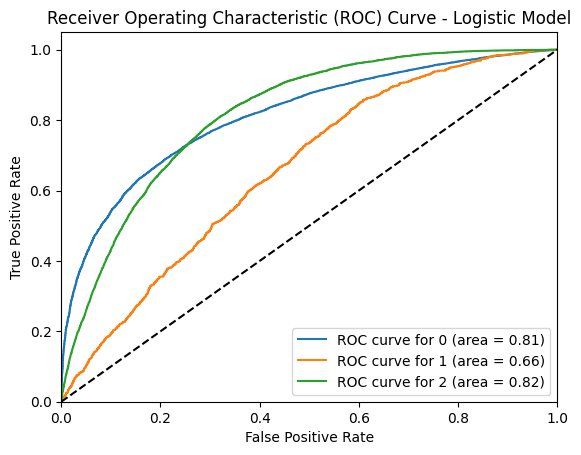
\includegraphics[scale=0.39]{logROC.png}
        \label{fig:logROC}
        \caption{Logistic Regression ROC}
    \end{figure}
    
    \begin{figure}[h]
        \centering
        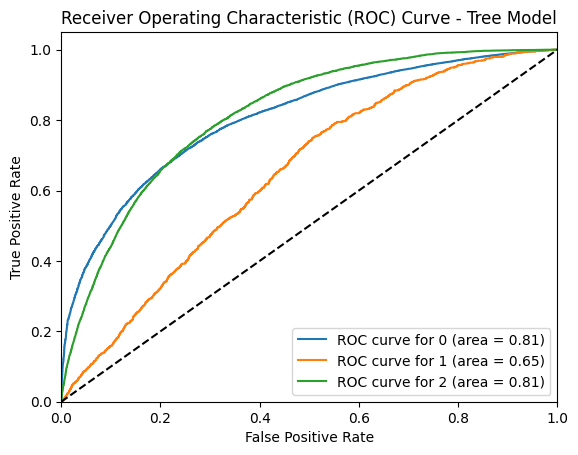
\includegraphics[scale=0.39]{treeROC.png}
        \label{fig:treeROC}
        \caption{XGBoost ROC}
    \end{figure}

    \begin{figure}[h]
        \centering
        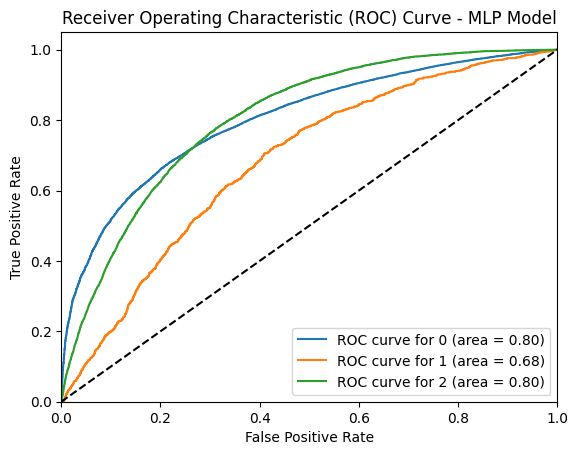
\includegraphics[scale=0.39]{ffnnROC.png}
        \label{fig:ffnnROC}
        \caption{DNN ROC}
    \end{figure}

    \begin{figure}[h]
        \centering
        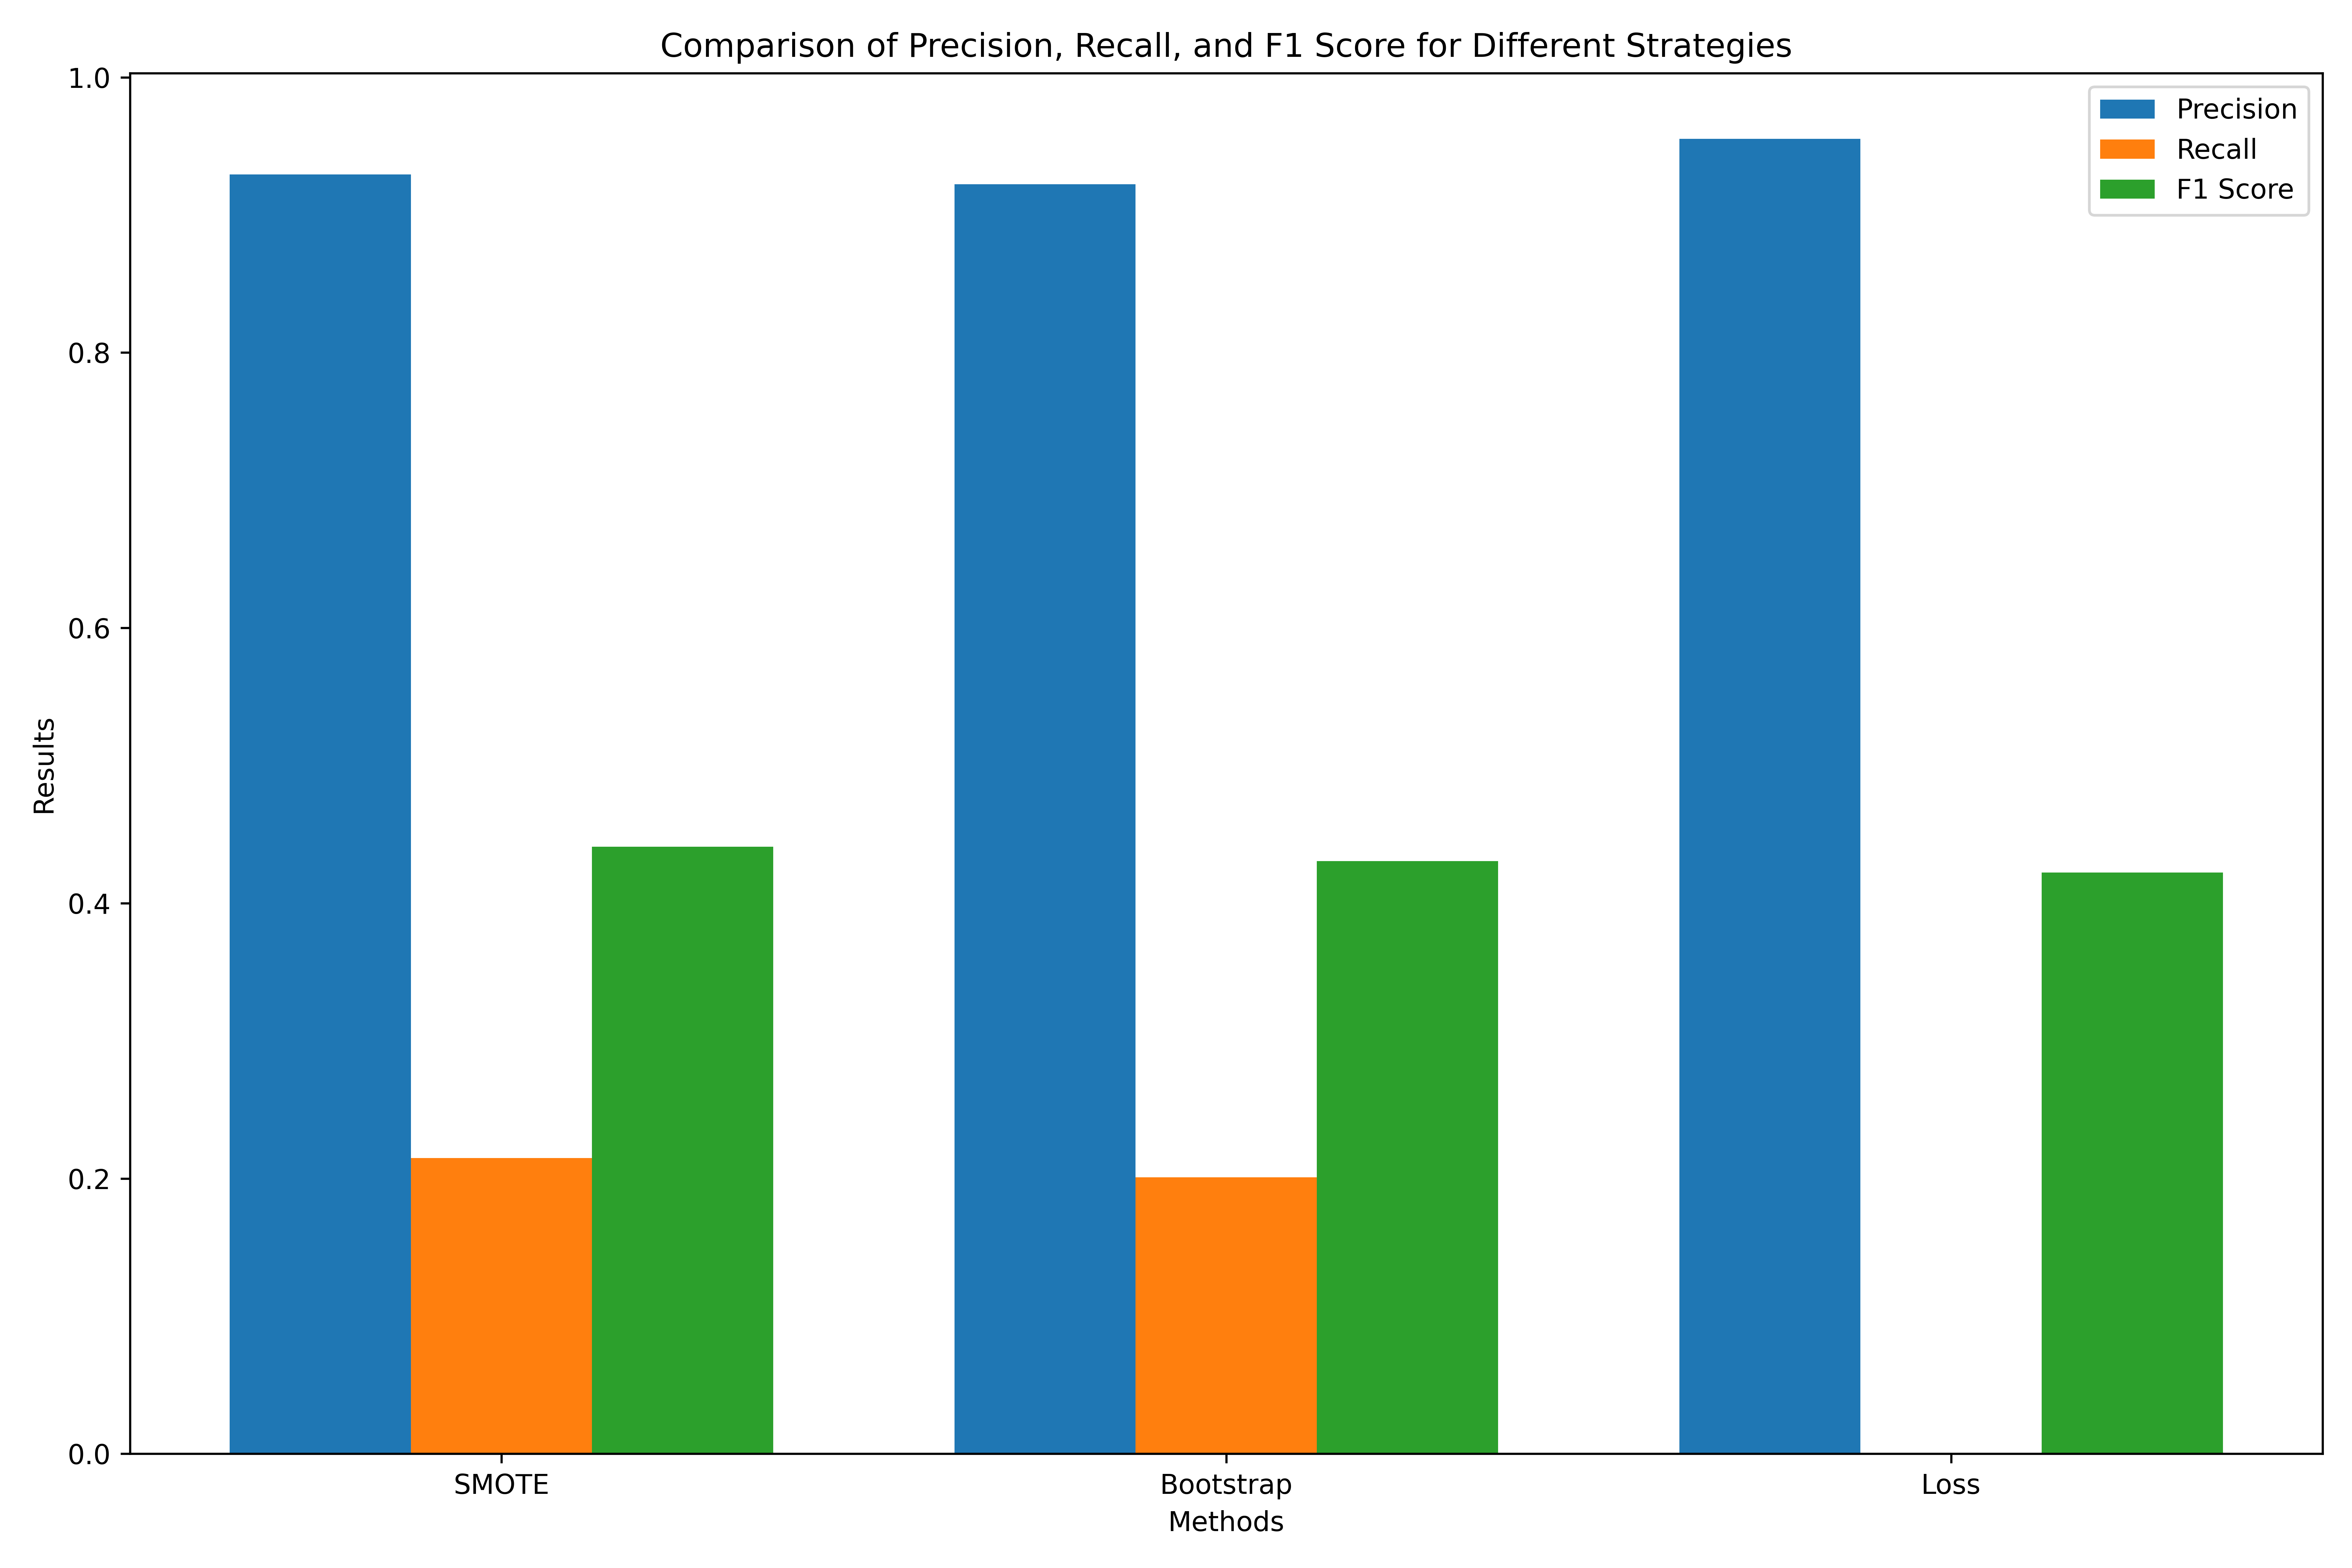
\includegraphics[scale = 0.30]{stratcomparison_high_dpi.png}
        \label{fig:stratcomparison}
        \caption{Class imbalance handling techniques}
    \end{figure}

    % \subsection{Logistic Model Results}
    % \begin{itemize}
    %     \item \textbf{Precision}: The logistic model shows high precision for 
    %     class 0 (Diabetes-Free) at 0.957, but lower precision for class 1 
    %     (pre-diabetes) and class 2 (diabetes). The precision is especially low for 
    %     class 2 at just 0.028. This can indicate a high number of false positives 
    %     for class 2 (diabetes).
        
    %     \item \textbf{Recall}: The recall for class 1 (pre-diabetes) is highest 
    %     among the classes at 0.649, compared to 0.601 for class 0 and 0.301 for 
    %     class 2. Again, the class 2 result is the lowest. This can indicate that 
    %     the model failed to predict true positive cases for the diabetes class.
        
    %     \item \textbf{F1-Score}: The F1-scores are highest for class 0 (0.743), 
    %     lower for class 1 (0.440), and extremely low (relatively speaking) for 
    %     class 2 (0.052), which is similar to the trend shown by precision and 
    %     recall.
        
    %     \item \textbf{Accuracy}: The logistic model has an overall accuracy of 
    %     60.791\%, which is relatively low compared to the other models. This can 
    %     indicate a difficulty in predicting the classes, specifically with classes 
    %     1 and 2, based on the above metrics.
        
    %     \item \textbf{AUC}: The AUC values for classes 0 and 2 (Diabetes-Free and 
    %     diabetes) are similar (0.81 and 0.82 respectively). For class 1 (pre-
    %     diabetes), the AUC is relatively lower at 0.66, indicating a difficulty in 
    %     distinguishing for this class.
    % \end{itemize}

    % \subsection{Decision Tree Model Results}
    % \begin{itemize}
    %     \item \textbf{Precision}: The Decision Tree model shows high precision for 
    %     class 0 (Diabetes-Free) at 0.941, but lower precision for class 1 
    %     (pre-diabetes) and class 2 (diabetes). The precision is especially low for 
    %     class 2 at just 0.028. This can indicate a high number of false positives 
    %     for class 2 (diabetes).
        
    %     \item \textbf{Recall}: The recall scores for class 0 (Diabetes-Free) and 
    %     class 1 (pre-diabetes) are somewhat similar (0.690 and 0.636 
    %     respectively). For class 2 (diabetes), the recall is relatively lower at 
    %     0.187.
        
    %     \item \textbf{F1-Score}: The F1-scores are highest for class 0 (0.796), 
    %     lower for class 1 (0.444), and extremely low (relatively speaking) for 
    %     class 2 (0.049), which is similar to the trend of F1-scores in the 
    %     logistic model.
        
    %     \item \textbf{Accuracy}: The Decision Tree model has an overall accuracy 
    %     of 67.341\%, which is substantially higher than the logistic model 
    %     accuracy (though lower than that of FFNN). This can indicate that the 
    %     Decision Tree model struggled less in predicting the classes compared to 
    %     the logistic model.
        
    %     \item \textbf{AUC}: The AUC values for classes 0 and 2 (Diabetes-Free and 
    %     diabetes) are both 0.81. For class 1 (pre-diabetes), the AUC is relatively 
    %     lower at 0.65, indicating a difficulty in distinguishing for this class. 
    %     This is a very similar trend to the AUC values for the logistic model.
    % \end{itemize}

    % \subsection{FFNN (Feedforward Neural Network) Model Results}
    % \begin{itemize}
    %     \item \textbf{Precision}: Like the other models, class 0 has the highest 
    %     precision by a wide margin at 0.933. However, opposite to the other 
    %     models, class 1 has a much lower precision compared to class 2 (0.035 and 
    %     0.314 respectively).
        
    %     \item \textbf{Recall}: Unlike other models, where class 1 has a 
    %     significantly lower recall (0.092) than class 2 (0.656). Like the other 
    %     models, class 0 is the highest at 0.732, though the difference between 
    %     class 0 and class 2 is much closer than other models. 
        
    %     \item \textbf{F1-Score}: Similar to prevision and recall, but unlike other 
    %     models, class 1 exhibits an extremely low result (0.050) compared to 
    %     classes 0 (0.821) and 2 (0.425). Class 0 leads with a margin similar to 
    %     that of the other models.
        
    %     \item \textbf{Accuracy}: The FFNN model exhibits the highest overall 
    %     accuracy among the three models at 70.983\%, which is an almost 10\% 
    %     increase over the logistic model and slightly better than the decision 
    %     tree model. This can indicate that the FFNN model struggled the least in 
    %     predicting the classes compared to the other models.
        
    %     \item \textbf{AUC}: The AUC values for classes 0 and 2 (Diabetes-Free and 
    %     diabetes) are both 0.80, similar to the decision tree and logistic models. 
    %     Again, for class 1 (pre-diabetes), the AUC is relatively lower at 0.68, 
    %     indicating a difficulty in distinguishing for this class.
    % \end{itemize}

    \subsection{Analysis}
        \begin{itemize}
            \item \textit{Precision, Recall, \& F1-Score}: As given by Table \ref{tab:results}, the Logistic and XGBoost (Gradient Boosting) models have relatively higher precision and recall for the Diabetes-Free label ($\sim$0.96, $\sim$0.94 respectively) compared to the positive classes. However, these models seemingly blanket predict Diabetes-Free as implied by their low precision but relatively higher recall scores in the positive labels (Pre-Diabetes, Diabetes). The Logistic model is most guilty of this, with a very high precision but a significantly lower recall ($\sim$0.61) for the Diabetes-Free label in comparison to the XGBoost model ($\sim$0.69) and certainly the Deep Neural Network [DNN] model ($\sim$0.93 precision, $\sim$0.73 recall).

            In comparison, the DNN seems to have learned the best about what is and isn't a Diabetes-Free label. Although the performance in the positive labels is quite mixed, implying that there's a fine-line between Pre-Diabetes and Diabetes patients in terms of their health metrics, the DNN does the best with regards to deciding between a negative versus positive label. In other words, the implication here is that if this were converted to a binary classification problem, the DNN would perform very well since it is very confident with its negative predictions.

            \item \textit{Accuracy}: although the class imbalance discourages the use of accuracy, the need to consistently predict well drives the use of accuracy as a background metric (i.e. something to consider, but not rely on for choosing a model).

            The DNN achieves the highest accuracy of $\sim$71\%, followed closely by the XGBoost model ($\sim$67\%) and further away the Logistic model ($\sim$61\%).

            The implication is of course that the Diabetes model, given a random subset of the population, will correctly identify roughly 71\% of people in the sample. Although this is lower than expected, prior experiments with this dataset failed to differentiate at all between the labels; most of the predictors instead blanket predicted a negative label, already gathering an 84\% accuracy due to imbalance. In the pursuit of remedying this, accuracy was one of the tradeoffs necessary to make (i.e. to learn more about the positive labels, we had to forgo accuracy).

            \item \textit{AUC}: area-under-curve, in reference to the ROC curve, is a scale and threshold invariant classification metric. As such, its primary utility for our purposes was to serve as another metric for  model selection. All models exhibit similar AUC values label-wise, but the DNN does outperform all other models in its consistency across labels.

            Generally, all models struggle the worst with the Pre-Diabetes label, thus showcasing the downstream effect of imbalance.
        \end{itemize}

    \subsection{Model Comparison}
    We observe then a trend among the models: DNN learned the most about the dataset as showcased by its superior consistency across labels and greater predictive ability, although all models suffered for the Pre-Diabetes label due to a major imbalance. More specifically, the better performing models (XGBoost, DNN) failed to learn meaningful ways to differentiate between the two positive labels (Pre-Diabetes and Diabetes), while the Logistic model failed to adequately learn the difference between the negative and positive labels at all.

    \subsection{Trends in Diabetes Risk}
    \begin{table}[h!]
        \centering
        \caption{Feature importance as measured by coefficient weight via Linear Approximation for Deep Learner. Negative indicates increase in risk of diabetes, magnitude indicates importance.}
        \label{tab:feature_importance}
        \begin{tabular}{l r}
            \toprule
            \textbf{Feature} & \textbf{Importance} \\
            \midrule
            Physical Health & 0.1437 \\
            Education & 0.0806 \\
            Heavy Drinker & 0.0599 \\
            Fruits & 0.0401 \\
            Income & 0.0226 \\
            Mental Health & 0.0150 \\
            Physical Activity & 0.0046 \\
            Smoker & 0.0000 \\
            Stroke & 0.0000 \\
            Heart Disease & 0.0000 \\
            Veggies & 0.0000 \\
            Healthcare & 0.0000 \\
            Difficulty Walking & 0.0000 \\
            Sex & -0.0249 \\
            No Doctor Because of Cost & -0.0512 \\
            Cholesterol Check & -0.1513 \\
            High Blood Pressure & -0.2333 \\
            High Cholesterol & -0.3341 \\
            BMI & -0.4028 \\
            Age & -0.4074 \\
            General Health & -0.6399 \\
            \bottomrule
        \end{tabular}
    \end{table}

    As Table \ref{tab:feature_importance} showcases, there certainly exists strong differences in the utility each feature provides the model. Prior to analysis, we want to emphasize that features are \textit{normalized} prior to prediction, i.e. the weights shown are for normalized values. Thus, the interpretability of these weights stays high, even with a large proportion of ordinal and nominal features.
    
    Considering the predictive context, many of the feature-wise weighting decisions make logical sense. Namely, a large proportion of the non-overlapping/unique (recall, this model is regularized via Elastic-Net) features describing physical health are all taken into consideration, e.g Physical Health, Physical Activity, BMI, General Health, and more.

    More interestingly, features not normally associated with Diabetes such as Education, Mental Health, Income, Heavy Drinker, and No Doctor Because of Cost all share interesting relationships with the risk prediction. Specifically, higher levels of education and income tend to reduce risk of diabetes, which could be due to increased knowledge of health and eating habits, higher tendencies to read newspapers and stay educated on the latest research, and most importantly access to healthier foods rather than lower quality fast foods. Most surprisingly, a worse Mental Health is actually associated with a lower risk of Diabetes, likely since stress has an inverse relationship with weight and weight gain for a large proportion of the population. This surprise continues with the Heavy Drinker feature also reducing risk of Diabetes. While this initially appears to conflict with initial predictions, it reveals a deeper truth about patient behavior--while some turn to sweet treats for celebration, others turn to alcohol. In this respect, the model may have inferred such a relationship exists with the patients in the dataset. Furthermore, the tendency to avoid visiting the doctor due to its cost likely prevents patients from taking action on their risk to a given disease (e.g. Diabetes), thus its negative impact on Diabetes becomes clear.

    However, conflicting observations are seen during case studies of the deep learner. Recall that we use the Logistic model to approximate the Deep Neural Network. While similar feature-wise trends are observed among both during experimentation and evaluation of user info towards downstream prediction, there appears to be strong conflicts with regards to some weightings. Most notably, the features Heart Disease and Stroke proved to be essential for the DNN to make its final prediction, on occasion being the difference between a Diabetes-Free and a Diabetes result. We conclude that this is expected behavior since the DNN is regularized via dropout, meaning it used all features in controlled quantities, unlike the regularized Logistic model which likely inferred the presence of Heart Disease and Stroke from features like Physical Health, Physical Activity, and General Health. Given the improved predictive power of the DNN, this likely proved to be a vital mistake for the Logistic model. More compelling, the reverse can also be possible--i.e. the DNN uses the occurrence of a Stroke and the presence of Heart Disease to infer the physical health of a patient.

    We claim that although there exist conflicts between the risk outlook from the deep learner versus the Logistic model, the end result utilizes the same feature information to make the end guess. It is worth noting that in future iterations, we could avoid regularization methods in the Logistic model to avoid such issues downstream in the risk prediction.

    Furthermore, we claim that we can generate an accurate prediction about a patient's pre-disposition to Diabetes with far fewer features than initially provided.

    \subsection{Evaluation Results and Discussion}
    Our experiments reveal that given an individual's lifestyle and subset of their biometrics, we can:
    \begin{enumerate}[label=\roman*.]
        \item identify their pre-disposition to Diabetes and approximate the risk factors that contribute to said disposition
        
        \item effectively distinguish between Diabetes-Free versus Pre-Diabetes/Diabetes patients, thus accomplishing two of the overarching research questions.
    \end{enumerate}

    While some limitations exist with regards to approximating the deep learner for risk evaluation and differentiating between the Pre-Diabetes/Diabetes classes, prior work [Kaggle] with the dataset outright failed to distinguish between any of the multi-class labels, relying on imbalance to boost accuracy.

    As previously stated, the models struggle the most with the insufficiency of Pre-Diabetes observations. While this certainly diminishes the models' ability to distinguish between the Pre-Diabetes and Diabetes labels, we claim that this inability is further aggrevated by the classes themselves being very close in this vector space (since blood sugar isn't one of the features and their meanings are quite similar). Given that SMOTE works via interpolation in the vector space with nearest neighbors, we hypothesize that the interpolation that SMOTE performs ends up combining the two labels' observations into an inseperable clump. Given the complexity of this visualization, we found it best to derive this through the upsampling breakdowns and downstream performances--i.e. look at the leaves to observe the wind.

    Most importantly, however, we claim that our system uses patient information accessible without labs, checkups, or other test results to give an approximation of their likelihood of Diabetes. Given such an information constraint and our goal of not necessarily predicting Diabetes, but rather determining whether a given patient has a pre-disposition to Diabetes that warrants further medical intervention, we conclude that we sufficiently provide patients with the risk information they desire. Thus, any patient regardless of financial, ethnic, religious, etc. background has access to the information they need without any barrier to entry.

    %TODO:: 
    %(1) given an individual’s lifestyle, can we identify specific risk factors for diabetes?
    %(2) Given an individual’s lifestyle, can we accurately assess whether they are diabetes-free, pre-diabetic, or diabetic?    
    

\section{Conclusion}\label{sec:conclusion}

    \begin{table*}[t]
        \centering
        \begin{tabular}{| c | c | c | c |}
            \toprule
            \textbf{Deliverable} & \textbf{Description} & \textbf{Due Date} & \textbf{Completion Date} \\ 
            \midrule
            Topic Selection & Select a problem to solve and determine how we will solve this problem. & 04/22 & 04/19 \\
            \midrule
            Topic Research & Research why a Diabetes classifier is important. & 04/22 & 04/21 \\
            \midrule
            Literature Review & Review other research papers that utilize ML for classification tasks & 05/05 & 05/03 \\
            \midrule
            EDA & Develop an understanding of our dataset. Pre-process where necessary. & 05/05 & 05/01 \\
            \midrule
            Feature Selection & Select the most important features to train our model. & 05/05 & 05/04 \\
            \midrule
            Model Construction and Testing & Create multiple models. Test the models and refine them accordingly. & 05/19 & 05/17 \\
            \midrule
            Model Evaluation and Selection & Evaluate and compare the models. Select the model that performs the best. & 05/26 & 05/28 \\
            \midrule
            Develop User Interface & Develop a front-end from where we can deploy our model. & 06/01 & 06/02 \\
            \midrule
            Complete Research Paper & Write and refine the research paper. & 06/08 & 06/07 \\
            \bottomrule
        \end{tabular}
        \vspace{0.2cm}
        \caption{Project Road-Map}
        \label{tab:roadmap}
    \end{table*}

In this paper, we claim that our Deep Neural Network classifier offers a balanced classification for individuals regarding diabetes (macro F1 score = 0.4251) and diabetes-free (F1-score 0.8206) classifications. However, the model struggles to identify individuals as pre-diabetic (F1 score = 0.0502). Therefore, we conclude that our model is effective for the binary classifications of diabetes and diabetes-free, but it falls short when we incorporate a pre-diabetes classification. Thus, in response to RQ \ref{itm:rq2}, we were able to find an effective solution, but ideally, we would find a way to raise our F1 score for pre-diabetes. Fortunately, the struggles we face with identifying pre-diabetes does not impact our ability to successfully answer RQ \ref{itm:rq1}. Although the model failed to classify pre-diabetes, our proficient classification of diabetes versus diabetes-free is sufficient enough to accurately decipher an individual’s risk factors. On all of our tests, the individual’s highlighted risk factors came in line with the risk factors we were expecting. As a result, the model was able to successfully identify risk factors in an individual given their lifestyle. However, since identifying risk factors is a relatively subjective test that primarily depends on the model weights, the success of the identification is heavily dependent on the effectiveness of our classifications. Therefore, if we utilized more advanced techniques to improve our model, it would likely lead to a more accurate identification of risk factors. \\
\indent The logical progression for this project would be to explore other approaches to create a more effective model. In a future implementation, it would be worthwhile to utilize advanced pre-processing techniques and remove the pre-diabetes classification. The scarcity of pre-diabetes samples likely confused our model and this issue was aggravated by upsampling. Because we initially did not have a representative sample of pre-diabetes, when we upsampled, we made our diabetes and diabetes-free samples less representative, thus removing the advantage of choosing a large dataset. Hence, if we focused on a diabetes vs. diabetes-free classifier, it would likely yield a more effective model. Additionally, considering more complicated modeling techniques like ensemble learning exist, they could also potentially increase our model’s effectiveness. Unfortunately, we had already committed to the modeling techniques we learned earlier in the quarter, so we were unable to test out the more complicated techniques discussed later on. However, incorporating these advanced techniques would likely generate more accurate and effective classifications. Hence, if we were to continue on this project, we should could improve on our model by removing the pre-diabetes label and leveraging more advanced techniques like ensemble learning.

\section{Project Roadmap, Repository, and Contributions}\label{sec:roadmap}

\subsection{Project Meta-Data}
\noindent For Project Roadmap refer to Table \ref{tab:roadmap}\\

\begin{itemize}
    \item \textit{Github}: \href{https://github.com/arjashok/ecs-171-project}{Project Link}
    
    \item \textit{Dataset}: \href{https://www.kaggle.com/datasets/alexteboul/diabetes-health-indicators-dataset}{Diabetes Health Indicators Dataset Link}
    
    \item \textit{Demo}: \href{https://youtu.be/DyyqayuNF2Y}{Project Demo}
\end{itemize}

\subsection{Author Contributions}
    \begin{itemize}
        \item \textit{Arjun Ashok*}: developed model architectures (DNN, XGBoost), model explainers \& risk analysis algorithms, package abstractions, package utilities, and strategies for downstream performance improvement; wrote Methodology, Experiments \& Evaluation
        
        \item \textit{Taha Abdullah}: assisted EDA with re-sampling; assisted with model prediction/evaluation by adding ROC/AUC; wrote portions of Literature Review and Evaluation Results and Discussion
        
        \item \textit{Tej Sidhu}: chose dataset using initial data selection metrics, researched diabetes and formulated our research questions, standardized the dataset, developed logistic regression model, developed front and back end, made project demo, and wrote Abstract, Introduction and Motivation, Conclusion, and Project Roadmap.

        \item \textit{Devon Streelman}: assisted EDA with outlier detection and visuals; wrote Abstract, Dataset \& Exploratory Data Analysis, Evaluation Results and Discussion; sourced and annotated research used in Literature Review
                
        \item \textit{Ayush Tripathi}: analyzed the dataset distributions and interpreted correlations within data; evaluated various class imbalance handling techniques by interpreting model performances; sourced research, condensed, and compiled literature review; compiled and formatted references. 
    \end{itemize}

\begin{thebibliography}{00}
\bibitem{b1} G. Eason, B. Noble, and I. N. Sneddon, ``On certain integrals of Lipschitz-Hankel type involving products of Bessel functions,'' Phil. Trans. Roy. Soc. London, vol. A247, pp. 529--551, April 1955.

\bibitem{b2} "Diabetes,” World Health Organization, \burl{https://www.who.int/news-room/fact-sheets/detail/diabetes#:~:text=Diabetes\%20is\%20a\%20chronic\%20disease,hormone\%20that\%20regulates\%20blood\%20glucose.}.(accessed Jun 5, 2024).

\bibitem{b3} G. Eason, B. Noble, and I. N. Sneddon, ``On certain integrals of Lipschitz-Hankel type involving products of Bessel functions,'' Phil. Trans. Roy. Soc. London, vol. A247, pp. 529--551, April 1955.

\bibitem{b4}
IDF Diabetes Atlas, \burl{https://diabetesatlas.org/#:~:text=Diabetes\%20around\%20the\%20world\%20in\%202021\%3A,\%2D\%20and\%20middle\%2Dincome\%20countries.} (accessed Jun. 5, 2024).

\bibitem{b5}I. Tasin, T. U. Nabil, S. Islam, and R. Khan, “Diabetes prediction using machine learning and explainable AI techniques,” Healthcare technology letters, 
\burl{https://www.ncbi.nlm.nih.gov/pmc/articles/PMC10107388/}. 

\bibitem{b6} J. P. Li, A. U. Haq, S. U. Din, J. Khan, A. Khan and A. Saboor, “Heart Disease Identification Method Using Machine Learning Classification in E-Healthcare,” IEEE Journals \& Magazine | IEEE Xplore, 2020. 

\burl{https://ieeexplore.ieee.org/document/9112202}

\bibitem{b7} R. Shwartz-Ziv and A. Armon, “Tabular data: Deep learning is not all you need,” Information Fusion, vol. 81, pp. 84–90, May 2022, doi: 
\burl{10.1016/j.inffus.2021.11.011}.

\burl{https://ieeexplore.ieee.org/document/9112202}.


\end{thebibliography}

\end{document}
